% =====================================================================
% PROPUESTA DE PROYECTO FINAL DE CARRERA -- v2
% Revisión tras observaciones de asesoría:
%   - pivote de dominio: LiDAR urbano  ->  patrimonio arquitectónico
%   - sección de ALCANCE separada y breve (datos, hardware, rangos)
%   - hipótesis eliminada
%   - diagrama con DOS BLOQUES (HyperNCD / Sonata) y FUSIÓN resaltada
%   - objetivos con resultado verificable; OE2 (integración) destacado
% Compilar: pdflatex propuesta_v2.tex  (x2)
% =====================================================================
\documentclass[9pt,twocolumn,a4paper]{extarticle}
\usepackage[utf8]{inputenc}
\usepackage[T1]{fontenc}
\usepackage[spanish,es-nodecimaldot,es-noshorthands]{babel}
\usepackage{times}
\usepackage{microtype}
\usepackage[a4paper,top=1.35cm,bottom=1.35cm,left=1.35cm,right=1.35cm,
            columnsep=0.55cm]{geometry}
\usepackage{amsmath,amssymb}
\usepackage{enumitem}
\usepackage{titlesec}
\usepackage{array}
\usepackage{booktabs}
\usepackage{xcolor}
\usepackage[hidelinks]{hyperref}
\usepackage[font=small,labelfont=bf,skip=2pt]{caption}
\usepackage{tikz}
\usetikzlibrary{arrows.meta,positioning,fit,calc,backgrounds}

\setlist{nosep,leftmargin=1.1em}
\setlength{\parindent}{1em}
\setlength{\parskip}{0pt}
\setlength{\abovedisplayskip}{3pt}
\setlength{\belowdisplayskip}{3pt}
\setlength{\intextsep}{4pt}
\setlength{\textfloatsep}{5pt}
\setlength{\dbltextfloatsep}{6pt}
\setlength{\floatsep}{4pt}
\setcounter{topnumber}{4}
\setcounter{totalnumber}{6}
\setcounter{dbltopnumber}{4}
\renewcommand{\topfraction}{0.98}
\renewcommand{\textfraction}{0.02}
\renewcommand{\floatpagefraction}{0.90}
\renewcommand{\dbltopfraction}{0.98}
\renewcommand{\dblfloatpagefraction}{0.90}
\titlespacing*{\section}{0pt}{6pt}{2pt}
\titleformat{\section}{\normalfont\bfseries}{\thesection}{0.5em}{}

% ------------------------- Paleta -------------------------
\definecolor{cIn}{HTML}{2563EB}     % entrada / datos
\definecolor{cPre}{HTML}{0891B2}    % preprocesamiento
\definecolor{cHyp}{HTML}{3A6EA5}    % BLOQUE 1 - HyperNCD
\definecolor{cSon}{HTML}{3A8D24}    % BLOQUE 2 - Sonata
\definecolor{cFus}{HTML}{D2691E}    % FUSIÓN (aporte)
\definecolor{cOut}{HTML}{6B21A8}    % salida
\definecolor{cDark}{HTML}{172033}

\tikzset{
  bx/.style={rectangle, rounded corners=5pt, align=center, font=\small,
             line width=1.1pt, inner sep=7pt, text=cDark},
  grp/.style={rectangle, rounded corners=10pt, dash pattern=on 5pt off 3pt,
              line width=1.1pt},
  tag/.style={rectangle, rounded corners=3pt, text=white,
              font=\bfseries\small, inner xsep=8pt, inner ysep=4pt},
  fl/.style={-{Latex[length=3.2mm,width=2.2mm]}, draw=cDark, line width=1.3pt},
  flf/.style={-{Latex[length=3.6mm,width=2.6mm]}, draw=cFus, line width=2.0pt},
  note/.style={font=\footnotesize\itshape, text=cDark!70}
}

\begin{document}
\pagestyle{empty}

\twocolumn[
\begin{center}
{\Large\bfseries Modelo híbrido HyperNCD--Sonata para el descubrimiento de
clases novedosas en la segmentación semántica de nubes de puntos de
patrimonio arquitectónico\par}
\vspace{3pt}
{\normalsize Renzo Felix Aponte \quad Manyory Cueva Mendoza\par}
\vspace{2pt}
{\small Escuela Profesional de Ingeniería de Sistemas / Ciencia de la
Computación --- UTEC\par}
\vspace{1pt}
{\small\itshape Propuesta de Proyecto Final de Carrera --- \today\par}
\end{center}
\vspace{3pt}
\begin{quotation}
\noindent\small\textbf{Resumen.}
La clasificación de elementos estructurales sobre nubes de puntos de
edificaciones patrimoniales ---distinguir columnas, arcos, bóvedas, cornisas
o contrafuertes dentro de un levantamiento con escáner láser--- se realiza
hoy de forma manual, elemento por elemento, porque no existe una herramienta
automatizada que cubra esa tarea. Los segmentadores semánticos 3D actuales no
la resuelven: operan bajo conjunto cerrado y fuerzan todo punto no previsto
hacia la clase conocida más cercana, un modo de falla inadmisible en un
edificio donde cada obra tiene elementos singulares. El paradigma
\emph{Novel Class Discovery} (NCD) levanta ese supuesto, pero su estado del
arte en 3D ---HyperNCD~\cite{hyperncd}--- alcanza solo 11.8--47.5 mIoU en
clases novedosas frente a 49.8 del modelo supervisado. Identificamos una
causa plausible: HyperNCD construye sus prototipos con descriptores
geométricos calculados a mano (linealidad, planaridad, \emph{scattering}).
Sonata~\cite{sonata} demostró que apoyarse en esas señales de bajo nivel
induce el \emph{geometric shortcut} y que corregirlo eleva el
\emph{linear probing} de 21.8\,\% a 72.5\,\% mIoU. Proponemos un
\textbf{modelo híbrido} que integra el \emph{encoder} auto-supervisado de
Sonata dentro del módulo de prototipos de HyperNCD, y cuantificamos la mejora
del mIoU sobre el levantamiento de la Catedral de Lima.
\vspace{2pt}

\noindent\small\textbf{Palabras clave:} nubes de puntos, segmentación
semántica 3D, \emph{novel class discovery}, aprendizaje auto-supervisado,
hipergrafos, patrimonio arquitectónico.
\end{quotation}
\vspace{4pt}
]

% =====================================================================
\section{Problema computacional}
% =====================================================================
Un levantamiento con escáner láser terrestre de una edificación patrimonial
produce una nube de puntos $P=\{(x_i,f_i)\}_{i=1}^{N}$ con miles de millones
de puntos y sin ninguna etiqueta semántica: el archivo sabe \emph{dónde} hay
materia, no \emph{qué} es. Para que ese levantamiento sirva a un ingeniero
civil ---análisis estructural, modelo BIM, informe de conservación--- alguien
debe asignar a cada punto la clase del elemento al que pertenece. Hoy ese
trabajo se hace \textbf{manualmente}: el especialista recorre el modelo,
selecciona regiones y las etiqueta una por una. No existe un software que lo
automatice, y ese vacío es el que este proyecto busca cubrir.

\textbf{Por qué en 3D y no sobre imágenes.} Un clasificador de imágenes
resuelve mal esta tarea porque su predicción depende del ángulo de captura y
de la iluminación: la misma columna fotografiada de frente y en escorzo
produce descriptores distintos. La nube de puntos codifica la geometría del
elemento de forma independiente del punto de vista, que es exactamente la
propiedad que el problema exige.

\textbf{Por qué la segmentación semántica estándar no basta.} Los métodos
actuales resuelven bien la tarea en dominios cerrados ---PTv3~\cite{ptv3}:
77.5 mIoU; Sonata: 79.4 mIoU en ScanNet--- pero comparten una restricción:
\emph{el conjunto de clases se fija durante el entrenamiento}. Un elemento no
previsto no se marca como desconocido, sino que se fuerza a la clase conocida
más parecida. En patrimonio esa restricción es fatal: cada edificio incorpora
elementos que no aparecen en ningún catálogo previo.

\textbf{El marco correcto: NCD.} Introducido a nubes de puntos por Riz
\emph{et al.}~\cite{nops}, el \emph{Novel Class Discovery} formaliza el
problema: dado $\mathcal{C}_k$ (clases conocidas, etiquetadas) y
$\mathcal{C}_n$ (clases novedosas, sin etiqueta), el modelo debe segmentar
ambas. Es la capacidad de \emph{detectar formas nuevas} sin haberlas visto
etiquetadas. El estado del arte, HyperNCD~\cite{hyperncd}, modela
asociaciones de alto orden mediante un hipergrafo de prototipos
geométrico-conscientes, donde cada punto se representa como
$F_i=[f_{\mathrm{sem}}(x^i);f_{\mathrm{geo}}(x^i)]$ (Ec.~3 de~\cite{hyperncd})
y $f_{\mathrm{geo}}$ se calcula analíticamente sobre los $k$NN ($k{=}15$).

\textbf{La debilidad explotable.} HyperNCD rinde entre 11.8 y 47.5 mIoU en
clases novedosas frente a 49.8 del supervisado: el modelo es débil justo
donde debería ser fuerte. Sonata~\cite{sonata} identifica una causa
candidata, el \emph{geometric shortcut}: la representación colapsa sobre
pistas geométricas accesibles (normales, altura) en lugar de aprender
semántica. Cuantificado por \emph{linear probing} en ScanNet: PointContrast
5.6\,\%, MSC 21.8\,\%, Sonata 72.5\,\% mIoU. HyperNCD construye su módulo
central precisamente sobre el tipo de descriptor que Sonata caracteriza como
problemático. Ambos trabajos nunca se han conectado.

\textbf{Propuesta.} Un \textbf{modelo híbrido}: conservar íntegro el
razonamiento por hipergrafo de HyperNCD y sustituir su rama geométrica manual
por las representaciones aprendidas del \emph{encoder} congelado de Sonata,
de modo que $F_i=[f_{\mathrm{sem}}(x^i);f_{\mathrm{ssl}}(x^i)]$. La mejora
esperada es de \emph{métrica}: un mIoU más alto sobre las clases novedosas se
traduce directamente en menos corrección manual por parte del ingeniero, que
es la condición para que la herramienta tenga valor práctico.

% ============ FIGURA: DIAGRAMA DE DISEÑO ==============
\begin{figure*}[!t]
\centering
\centering
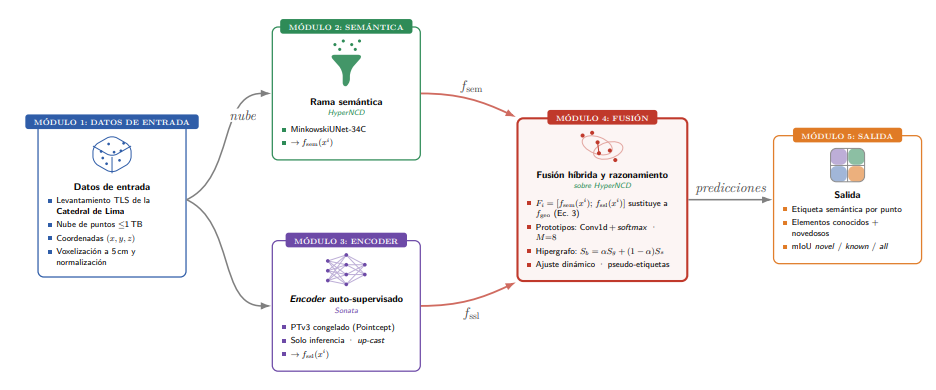
\includegraphics[width=\linewidth]{imagenes/grafico.png}

\caption{modulos}
\label{fig:catedral}

\caption{\textbf{Diagrama de diseño del sistema propuesto.} 
La nube TLS de la
Catedral de Lima (Módulo~1) alimenta en paralelo dos ramas de extracción: la
rama semántica MinkowskiUNet-34C de \textbf{HyperNCD} (Módulo~2), que produce
$f_{\mathrm{sem}}$, y el \emph{encoder} PTv3 preentrenado de \textbf{Sonata}
(Módulo~3), congelado y usado solo en inferencia, que produce
$f_{\mathrm{ssl}}$. Ambos descriptores entran al Módulo~4, donde reside el
aporte de la tesis: la concatenación
$F_i=[f_{\mathrm{sem}}(x^i);f_{\mathrm{ssl}}(x^i)]$ reemplaza al descriptor
geométrico manual $f_{\mathrm{geo}}$ (Ec.~3 de HyperNCD) antes de la formación
de prototipos y del razonamiento por hipergrafo, que permanecen intactos, de
modo que la variación de la métrica sea atribuible al reemplazo.}
\label{fig:diseno}
\end{figure*}

% =====================================================================
\section{Alcance}
% =====================================================================
\textbf{Objeto de estudio.} Un único edificio nombrado, la \textbf{Catedral
de Lima}, a partir del levantamiento provisto por la Facultad de Ingeniería
Civil. No se evalúan varias edificaciones distintas para escoger cuál
funciona mejor: el objeto es fijo y el modelo se ajusta a él, seccionado en
subconjuntos espaciales (nave, crucero, ábside, torres, fachada).

\textbf{Generalización declarada.} Los resultados se declaran válidos para
estructuras de tipología \emph{catedral / iglesia colonial} ---nave con
columnas y arcos, cubierta abovedada, fachada con torres--- y no se extienden
a vivienda, infraestructura vial ni obra industrial.

\textbf{Volumen de datos.} Tope de \textbf{1\,TB} de nube bruta. La
Tabla~\ref{tab:comp} detalla la cadena de reducción; el vóxel de 5\,cm es el
parámetro que hace el problema tratable y por eso se declara como límite, no
como preferencia. Reducir la nube por debajo de ese volumen efectivo
comprometería la significancia del resultado: con muy pocos puntos por clase
novedosa la diferencia entre el modelo base y el híbrido deja de ser
distinguible del ruido entre corridas.

\textbf{Hardware.} El proyecto está limitado por cómputo y así se declara. La
ejecución de referencia es sobre el clúster \textbf{Khipu} (UTEC); el
respaldo es una GPU dedicada de $\geq$12\,GB de VRAM, sobre la que el plan
sigue siendo viable pero con un tiempo de calendario aproximadamente un orden
de magnitud mayor. El seccionamiento de la catedral es precisamente el
mecanismo que permite ese respaldo: ninguna etapa requiere la nube completa
en memoria.

\begin{table}[t]
\centering
\small
\setlength{\tabcolsep}{4pt}
\caption{Presupuesto de datos y cómputo. Estimación de orden de magnitud bajo
los supuestos indicados; a confirmar contra el levantamiento real.}
\label{tab:comp}
\begin{tabular}{@{}p{3.0cm}p{2.1cm}p{2.4cm}@{}}
\toprule
\textbf{Etapa} & \textbf{Volumen} & \textbf{Cómputo} \\
\midrule
Nube bruta (TLS) & $\leq$1\,TB, $\sim$3$\times$10$^{10}$ pts & almacenamiento \\
Teselado por secciones ($n{\approx}8$) & $\sim$125\,GB / sección & CPU \\
Vóxel 5\,cm ($\sim$5$\times$10$^{4}$\,m$^2$ de superficie) & $\sim$2$\times$10$^{7}$ pts & 1 GPU \\
Ventana por paso & $\sim$10$^{5}$ pts & 12--24\,GB VRAM \\
Sonata congelado (1 pasada, \emph{cache}) & fija & $\sim$2 GPU-h \\
Corrida de entrenamiento & --- & $\sim$10 GPU-h \\
\midrule
\textbf{Total del plan} ($\sim$30 corridas) & --- & \textbf{$\sim$300 GPU-h} \\
\bottomrule
\end{tabular}
\end{table}

Con ese presupuesto, \textbf{Khipu es suficiente}: 300 GPU-h se cubren en
pocos días con asignación multi-GPU, mientras que una GPU aislada requeriría
del orden de dos semanas de cómputo continuo.

\textbf{Rangos de operación.} El proyecto declara por adelantado dónde se
espera que el método funcione y dónde no; OE4 los verifica empíricamente.

\emph{Rango favorable:} densidad efectiva $\geq$1\,pt/cm$^2$ tras
voxelización; elementos de escala $\geq$20\,cm con firma geométrica repetida
(columnas, arcos, bóvedas, cornisas, contrafuertes); cobertura
$\geq$70\,\% de la superficie del elemento; hasta $\sim$6 clases novedosas
por sección.

\emph{Rango desfavorable:} ornamento fino ($<$5\,cm), por debajo de la
resolución del vóxel; superficies con oclusión severa o escaneadas desde un
único ángulo; clases novedosas con menos de $\sim$0.5\,\% de los puntos de la
sección ---régimen en el que HyperNCD ya colapsa (11.8 mIoU en el
\emph{split} 3 de SemanticKITTI); número elevado de clases simultáneas, donde
la representación de Sonata pierde discriminación (29.3 mIoU en ScanNet200,
200 clases, frente a 72.5 en ScanNet, 20 clases); y elementos definidos por
material o color más que por geometría.

\textbf{Excluye:} preentrenamiento auto-supervisado propio (Sonata requirió
140k escenas y 32 GPU); detección de instancias; vocabulario abierto basado
en modelos de lenguaje; ejecución en tiempo real; generación del modelo BIM
aguas abajo de la segmentación.

% =====================================================================
\section{Diseño de proyecto}
% =====================================================================
La Fig.~\ref{fig:diseno} organiza el sistema en \textbf{dos bloques
metodológicos} y un \textbf{punto de fusión}. El Bloque~1 es HyperNCD: aporta
la rama semántica (MinkowskiUNet-34C) y toda la maquinaria de prototipos,
hipergrafo dinámico y pseudo-etiquetas que permite descubrir clases nuevas.
El Bloque~2 es Sonata: un \emph{encoder} PTv3 preentrenado de forma
auto-supervisada, usado con pesos congelados y solo en inferencia. El nodo de
fusión es el aporte de la tesis: allí, y solo allí, se sustituye
$f_{\mathrm{geo}}$ por $f_{\mathrm{ssl}}$ antes de la formación de
prototipos.

Al mover una sola pieza, cualquier variación de la métrica es atribuible al
reemplazo, lo que hace la ablación interpretable sin ambigüedad. Aguas abajo
de la fusión, la afinidad entre prototipos sigue combinando componente
geométrica y semántica, $S_b=\alpha S_g+(1-\alpha)S_s$ con $\alpha\in[0,1]$,
y cada prototipo conserva sus $M{=}8$ vecinos al construir el hipergrafo.

\textbf{Ventaja de dominio del pivote.} Sonata se preentrenó sobre escenas
interiores densas (ScanNet, S3DIS, Structured3D, HM3D). En LiDAR urbano
exterior su \emph{linear probing} queda por debajo de PTv3 entrenado desde
cero (62.0 frente a 69.1 mIoU en SemanticKITTI), pero en interiores
arquitectónicos densos alcanza 72.5 mIoU en ScanNet y 72.3 en S3DIS Área 5,
a la par de modelos supervisados completos. El levantamiento de una catedral
---estático, denso, de geometría arquitectónica--- cae del lado favorable de
esa frontera. El principal riesgo declarado en versiones previas de esta
propuesta se reduce sustancialmente con el cambio de dominio.

\textbf{Riesgo y mitigación.} Persisten dos. (i)~\emph{Anotación}: NCD exige
al menos las clases conocidas etiquetadas; se asume la anotación manual de
una sección de referencia con $\geq$4 clases base, y si el levantamiento
llega sin etiquetas esa anotación se vuelve tarea previa del cronograma.
(ii)~\emph{Sustitución vs.\ concatenación}: si el reemplazo directo degrada,
el Plan~B es concatenar,
$F_i=[f_{\mathrm{sem}};f_{\mathrm{geo}};f_{\mathrm{ssl}}]$, dejando que el
módulo de prototipos pondere las tres fuentes. Cualquier resultado
---mejora, paridad o degradación--- documentado con ablación es reportable.


% =====================================================================
\section{Objetivos}
% =====================================================================
\textbf{Objetivo general.} Construir y medir un modelo híbrido que integre
las representaciones auto-supervisadas de Sonata en el módulo de prototipos
de HyperNCD, y cuantificar la mejora del mIoU en la clasificación de
elementos estructurales no anotados sobre el levantamiento de la Catedral de
Lima.

\textbf{OE1 --- Establecer la línea base.} Reproducir HyperNCD sin
modificaciones sobre las secciones anotadas de la catedral, con tres corridas
independientes. \emph{Herramientas:} Python 3.10, PyTorch, MinkowskiEngine,
código oficial de HyperNCD, MinkowskiUNet-34C. \emph{Resultado verificable:}
tabla de mIoU \emph{novel}\,/\,\emph{known}\,/\,\emph{all} por sección, con
desviación estándar reportada.

\textbf{OE2 --- Integrar Sonata en el módulo de prototipos
\textnormal{(objetivo central)}.} Implementar el bloque de fusión que
sustituye $f_{\mathrm{geo}}$ por $f_{\mathrm{ssl}}$ en la Ec.~3 de HyperNCD,
inmediatamente antes de la asignación suave a prototipos, resolviendo la
compatibilidad de resolución entre el \emph{encoder} PTv3 y la rejilla de
Minkowski mediante \emph{up-cast} y \emph{cache} de características por
sección. \emph{Herramientas:} pesos públicos de Sonata, Pointcept, PTv3,
\texttt{spconv}. \emph{Resultado verificable:} repositorio con el modelo
híbrido corriendo de extremo a extremo y produciendo
$F_i=[f_{\mathrm{sem}};f_{\mathrm{ssl}}]$, con las dimensiones de ambas ramas
documentadas.

\textbf{OE3 --- Calibrar la configuración del híbrido.} Determinar los
valores de $\alpha$ (balance geométrico-semántico), $M$ (vecinos por
hiperarista) y $\epsilon$ (suavizado de etiquetas) que maximizan el mIoU
\emph{novel} en una sección de referencia. \emph{Herramientas:} búsqueda por
grilla acotada, AdamW, Weights\,\&\,Biases. \emph{Resultado verificable:}
curvas de sensibilidad de los tres parámetros y configuración fijada, luego
aplicada sin reajuste al resto de secciones.

\textbf{OE4 --- Cuantificar la mejora y delimitar el rango de operación.}
Medir $\Delta$mIoU del híbrido frente a la línea base de OE1, aislar la
contribución del \emph{encoder} mediante tres variantes (geométrica manual /
auto-supervisada / concatenada), y determinar empíricamente la frontera entre
el rango favorable y el desfavorable declarados en la Sec.~2, barriendo
densidad de puntos, tamaño de sección y número de clases novedosas.
\emph{Herramientas:} mIoU con emparejamiento húngaro, visualizaciones PCA.
\emph{Resultado verificable:} tabla comparativa, estudio de ablación y curva
de degradación que fija el rango declarado.

% =====================================================================
\section{Resultados esperados}
% =====================================================================
El resultado central es un \textbf{incremento medible del mIoU sobre las
clases novedosas} respecto de HyperNCD sin modificar, sin degradación de las
clases conocidas. Ese número es el que interesa al ingeniero civil: cada
punto de mIoU adicional es trabajo manual de corrección que deja de
realizarse. Los usuarios están conformes con la precisión que obtienen hoy
por vía manual, de modo que la propuesta de valor no es igualarla sino
automatizarla a una precisión suficiente; sin mejora demostrada sobre el
estado del arte, la herramienta no tiene caso.

Entregables: (i)~línea base reproducida con desviación reportada (OE1);
(ii)~implementación del modelo híbrido y repositorio público (OE2);
(iii)~curvas de sensibilidad de $\alpha$, $M$ y $\epsilon$ (OE3);
(iv)~tablas comparativas, ablación de tres variantes y frontera de operación
declarada (OE4).

La contribución al estado del arte no es una arquitectura nueva sino
establecer si un hallazgo demostrado en régimen supervisado ---la nocividad
del \emph{geometric shortcut}--- se transfiere al régimen de descubrimiento
de clases novedosas, donde la calidad de la representación es más crítica
porque no hay supervisión sobre las clases objetivo. Es un resultado
incierto, medible y no reportado por ningún trabajo previo: exactamente la
condición que justifica investigarlo. Bajo el Plan~B de la Sec.~3, incluso un
resultado nulo o negativo, documentado con ablación, constituye un hallazgo
reportable.

{\small
\begin{thebibliography}{9}
\bibitem{nops} L. Riz, C. Saltori, E. Ricci y F. Poiesi, ``Novel Class
Discovery for 3D Point Cloud Semantic Segmentation'', \emph{CVPR}, 2023.
\bibitem{ptv3} X. Wu \emph{et al.}, ``Point Transformer V3: Simpler, Faster,
Stronger'', \emph{CVPR}, 2024.
\bibitem{dasl} R. Xu, C. Zhang, H. Ren y X. He, ``Dual-Level Adaptive
Self-Labeling for Novel Class Discovery in Point Cloud Segmentation'',
\emph{ECCV}, 2024.
\bibitem{sonata} X. Wu \emph{et al.}, ``Sonata: Self-Supervised Learning of
Reliable Point Representations'', \emph{arXiv:2503.16429}, 2025.
\bibitem{hyperncd} Z. Zhang, A. Wu, Y. Li, Y. Han y J. Shen,
``Geometric-Aware Hypergraph Reasoning for Novel Class Discovery in Point
Cloud Segmentation'', \emph{arXiv:2606.07280}, 2026.
\end{thebibliography}}

\end{document}
